% questions.tex —— 2010 年·普通高等学校招生考试·山东卷·文科 · 题目内容片段（无答案）
% 由 tools/generate_projects.py 依来源总账自 2010/2010_数学真题_山东文_试题.md 生成，勿手改（改源 MD 后重跑）


状态：needs-review；依固定候选 PDF 两页（印刷页 621–622）逐题核验，四幅图已矢量重绘。原页未印分值，不补。

\gkpart{一、选择题}

\begin{question}
\gkti{1}已知全集 $U=\mathbf R$，集合 $M=\{x\mid x^2-4\leqslant0\}$，则 $\complement_UM=$（　）

（A）$\{x\mid -2<x<2\}$

（B）$\{x\mid -2\leqslant x\leqslant2\}$

（C）$\{x\mid x<-2\text{ \text{或} }x>2\}$

（D）$\{x\mid x\leqslant-2\text{ \text{或} }x\geqslant2\}$

\end{question}
\begin{question}
\gkti{2}已知 $\dfrac{a+2\mathrm i}{\mathrm i}=b+\mathrm i$（$a,b\in\mathbf R$），其中 $\mathrm i$ 为虚数单位，则 $a+b=$（　）

（A）$-1$

（B）$1$

（C）$2$

（D）$3$

\end{question}
\begin{question}
\gkti{3}函数 $f(x)=\log_2(3^x+1)$ 的值域为（　）

（A）$(0,+\infty)$

（B）$[0,+\infty)$

（C）$(1,+\infty)$

（D）$[1,+\infty)$

\end{question}
\begin{question}
\gkti{4}在空间，下列命题正确的是（　）

（A）平行直线的平行投影重合

（B）平行于同一直线的两个平面平行

（C）垂直于同一平面的两个平面平行

（D）垂直于同一平面的两条直线平行

\end{question}
\begin{question}
\gkti{5}设 $f(x)$ 为定义在 $\mathbf R$ 上的奇函数，当 $x\geqslant0$ 时，$f(x)=2^x+2x+b$（$b$ 为常数），则 $f(-1)=$（　）

（A）$-3$

（B）$-1$

（C）$1$

（D）$3$

\end{question}
\begin{question}
\gkti{6}在某项体育比赛中，七位裁判为一选手打出的分数如下：$90$，$89$，$90$，$95$，$93$，$94$，$93$。去掉一个最高分和一个最低分后，所剩数据的平均分值和方差分别为（　）

（A）$92$，$2$

（B）$92$，$2.8$

（C）$93$，$2$

（D）$93$，$2.8$

\end{question}
\begin{question}
\gkti{7}设 $\{a_n\}$ 是首项大于零的等比数列，则“$a_1<a_2$”是“数列 $\{a_n\}$ 是递增数列”的（　）

（A）充分而不必要条件

（B）必要而不充分条件

（C）充分必要条件

（D）既不充分也不必要条件

\end{question}
\begin{question}
\gkti{8}已知某生产厂家的年利润 $y$（单位：万元）与年产量 $x$（单位：万件）的函数关系式为 $y=-\dfrac13x^3+81x-234$，则使该生产厂家获得最大年利润的年产量为（　）

（A）$13$ 万件

（B）$11$ 万件

（C）$9$ 万件

（D）$7$ 万件

\end{question}
\begin{question}
\gkti{9}已知抛物线 $y^2=2px$（$p>0$），过其焦点且斜率为 $1$ 的直线交抛物线于 $A$、$B$ 两点，若线段 $AB$ 的中点的纵坐标为 $2$，则该抛物线的准线方程为（　）

（A）$x=1$

（B）$x=-1$

（C）$x=2$

（D）$x=-2$

\end{question}
\begin{question}
\gkti{10}观察 $(x^2)'=2x$，$(x^4)'=4x^3$，$(\cos x)'=-\sin x$，由归纳推理可得：若定义在 $\mathbf R$ 上的函数 $f(x)$ 满足 $f(-x)=f(x)$，记 $g(x)$ 为 $f(x)$ 的导函数，则 $g(-x)=$（　）

（A）$f(x)$

（B）$-f(x)$

（C）$g(x)$

（D）$-g(x)$

\Needspace{0.4\textheight}
\end{question}
\begingroup
\renewenvironment{question}{\Needspace{0.5\textheight}}{}
\begin{question}
\gkti{11}函数 $y=2^x-x^2$ 的图象大致是（　）
\nopagebreak[4]
\begin{center}% 2010 年山东卷文科第 11 题：四个函数图象选项（A）—（D）。
% 来源 PDF：普通高考/2010/2010山东文.pdf，SHA-256 95a69b861a29ca594f9118c9643efcdfd04cae3c4f374ff9fa009f7ac99712f4。
% 原页：第 1 页（A3 三栏）第 2 栏上部，书页码 621。
% 重绘依据：正确图象为 y=2^x-x^2：x→-∞ 时 y→-∞，过负根后上升，x=0 时 y=1，
%   x=2 与 x=4 时 y=0，2<x<4 时 y<0，x>4 后上升。其余三幅为干扰项。
\begin{tikzpicture}[semithick, every node/.style={inner sep=1.2pt, font=\small}]
  % (A) 正确图象
  \begin{scope}
    \draw[-stealth] (-2.5,0) -- (5.0,0) node[right] {$x$};
    \draw[-stealth] (0,-1.6) -- (0,1.3) node[above] {$y$};
    \draw[thick,domain=-2.3:4.75,samples=180]
      plot (\x,{0.28*(exp(\x*ln(2))-(\x)*(\x))});
    \node at (1.2,-2.15) {（A）};
  \end{scope}
  % (B) 干扰项
  \begin{scope}[shift={(7.2,0)}]
    \draw[-stealth] (-2.3,0) -- (4.8,0) node[right] {$x$};
    \draw[-stealth] (0,-1.5) -- (0,1.6) node[above] {$y$};
    \draw[thick] (-2.2,-1.1) .. controls (-1.2,1.8) and (1.4,1.7) .. (3.6,0.05)
      .. controls (4.1,-0.1) and (4.4,0.5) .. (4.7,1.4);
    \node at (1.2,-2.15) {（B）};
  \end{scope}
  % (C) 干扰项
  \begin{scope}[shift={(0,-4.6)}]
    \draw[-stealth] (-2.2,0) -- (4.8,0) node[right] {$x$};
    \draw[-stealth] (0,-1.4) -- (0,1.6) node[above] {$y$};
    \draw[thick] (-2.1,1.2) .. controls (-1.2,-0.4) and (0.4,-0.2) .. (1.4,0.9)
      .. controls (2.2,1.6) and (2.8,0.9) .. (3.0,-0.1)
      .. controls (3.2,-1.0) and (3.5,-1.2) .. (3.9,-1.4);
    \node at (1.2,-2.15) {（C）};
  \end{scope}
  % (D) 干扰项
  \begin{scope}[shift={(7.2,-4.6)}]
    \draw[-stealth] (-2.2,0) -- (4.8,0) node[right] {$x$};
    \draw[-stealth] (0,-1.6) -- (0,1.5) node[above] {$y$};
    \draw[thick] (-2.1,0.7) .. controls (-1.4,-0.5) and (-0.8,0.4) .. (0.0,0.65)
      .. controls (0.9,0.9) and (1.1,-0.5) .. (1.5,-1.1)
      .. controls (2.1,-1.8) and (3.3,-0.3) .. (4.6,1.2);
    \node at (1.2,-2.15) {（D）};
  \end{scope}
\end{tikzpicture}
\end{center}
\nopagebreak[4]
\end{question}
\endgroup
\begin{question}
\gkti{12}定义平面向量之间的一种运算“$\odot$”如下：对任意的 $\boldsymbol a=(m,n)$，$\boldsymbol b=(p,q)$，令 $\boldsymbol a\odot\boldsymbol b=mq-np$。下面说法错误的是（　）

（A）若 $\boldsymbol a$ 与 $\boldsymbol b$ 共线，则 $\boldsymbol a\odot\boldsymbol b=0$

（B）$\boldsymbol a\odot\boldsymbol b=\boldsymbol b\odot\boldsymbol a$

（C）对任意的 $\lambda\in\mathbf R$，有 $(\lambda\boldsymbol a)\odot\boldsymbol b=\lambda(\boldsymbol a\odot\boldsymbol b)$

（D）$(\boldsymbol a\odot\boldsymbol b)^2+(\boldsymbol a\cdot\boldsymbol b)^2=|\boldsymbol a|^2|\boldsymbol b|^2$

\end{question}
\gkpart{二、填空题}

\Needspace{0.4\textheight}
\begingroup
\renewenvironment{question}{\Needspace{0.5\textheight}}{}
\begin{question}
\gkti{13}执行如图所示的程序框图，若输入 $x=4$，则输出 $y$ 的值为$\underline{\qquad}$。
\nopagebreak[4]
\begin{center}% 2010 年山东卷文科第 13 题：程序框图。
% 来源 PDF：普通高考/2010/2010山东文.pdf，SHA-256 95a69b861a29ca594f9118c9643efcdfd04cae3c4f374ff9fa009f7ac99712f4。
% 原页：第 1 页（A3 三栏）第 2 栏中部，书页码 621。
% 重绘依据：开始 → 输入 x → y=(1/2)x-1 → 判断 |y-x|<1；
%   是（下）→ 输出 y → 结束；否（右）→ x=y → 回到 y=(1/2)x-1 之前。
\begin{tikzpicture}[semithick, >=Stealth,
  every node/.style={inner sep=1.5pt, font=\small}]
  \node (start) [draw, rounded corners=4pt, minimum width=1.8cm, minimum height=0.55cm] at (0,0) {开始};
  \node (in) [draw, trapezium, trapezium left angle=72, trapezium right angle=108,
    minimum width=2.2cm, minimum height=0.55cm] at (0,-1.35) {输入 $x$};
  \node (calc) [draw, minimum width=2.6cm, minimum height=0.65cm] at (0,-2.9) {$y=\dfrac12x-1$};
  \node (test) [draw, diamond, aspect=2.2, minimum width=3.4cm, minimum height=1.25cm] at (0,-4.8) {$|y-x|<1$};
  \node (out) [draw, trapezium, trapezium left angle=72, trapezium right angle=108,
    minimum width=2.2cm, minimum height=0.55cm] at (0,-6.7) {输出 $y$};
  \node (end) [draw, rounded corners=4pt, minimum width=1.8cm, minimum height=0.55cm] at (0,-8.1) {结束};
  \node (assign) [draw, minimum width=1.5cm, minimum height=0.6cm] at (4.2,-2.9) {$x=y$};

  \draw[->] (start) -- (in);
  \draw[->] (in) -- (calc);
  \draw[->] (calc) -- (test);
  \draw[->] (test.south) -- node[right] {是} (out.north);
  \draw[->] (out) -- (end);
  \draw[->] (test.east) -- node[above] {否} (4.2,-4.8);
  \draw[->] (4.2,-4.8) -- (assign.south);
  \draw[->] (assign.north) -- (4.2,-1.7) -- (0,-1.7);
  \draw[->] (0,-1.7) -- (calc.north);
\end{tikzpicture}
\end{center}
\nopagebreak[4]
\end{question}
\endgroup
\begin{question}
\gkti{14}已知 $x,y\in\mathbf R_+$，且满足 $\dfrac x3+\dfrac y4=1$，则 $xy$ 的最大值为$\underline{\qquad}$。

\end{question}
\begin{question}
\gkti{15}在 $\triangle ABC$ 中，$A$，$B$，$C$ 所对的边分别为 $a$，$b$，$c$。若 $a=\sqrt2$，$b=2$，$\sin B+\cos B=\sqrt2$，则角 $A$ 的大小为$\underline{\qquad}$。

\end{question}
\begin{question}
\gkti{16}已知圆 $C$ 过点 $(1,0)$，且圆心在 $x$ 轴的正半轴上，直线 $l:y=x-1$ 被圆 $C$ 所截得的弦长为 $2\sqrt2$，则过圆心且与直线 $l$ 垂直的直线的方程为$\underline{\qquad}$。

\end{question}
\gkpart{三、解答题}

\begin{question}
\gkti{17}已知函数 $f(x)=\sin(\pi-\omega x)\cos\omega x+\cos^2\omega x$（$\omega>0$）的最小正周期为 $\pi$。

（1）求 $\omega$ 的值；

（2）将函数 $y=f(x)$ 的图象上各点的横坐标缩短到原来的 $\dfrac12$，纵坐标不变，得到函数 $y=g(x)$ 的图象，求函数 $y=g(x)$ 在区间 $\left[0,\dfrac\pi{16}\right]$ 上的最小值。

\end{question}
\begin{question}
\gkti{18}已知等差数列 $\{a_n\}$ 满足：$a_3=7$，$a_5+a_7=26$。数列 $\{a_n\}$ 的前 $n$ 项和为 $S_n$。

（1）求 $a_n$ 及 $S_n$；

（2）令 $b_n=\dfrac1{a_n^2-1}$（$n\in\mathbf N^*$），求数列 $\{b_n\}$ 的前 $n$ 项和 $T_n$。

\end{question}
\begin{question}
\gkti{19}一个袋中装有四个形状大小完全相同的球，球的编号分别为 $1,2,3,4$。

（1）从袋中随机取两个球，求取出的球的编号之和不大于 $4$ 的概率；

（2）先从袋中随机取一个球，该球的编号为 $m$，将球放回袋中，然后再从袋中随机取一个球，该球的编号为 $n$，求 $n<m+2$ 的概率。

\Needspace{0.4\textheight}
\end{question}
\begingroup
\renewenvironment{question}{\Needspace{0.5\textheight}}{}
\begin{question}
\gkti{20}在如图所示的几何体中，四边形 $ABCD$ 是正方形，$MA\perp$ 平面 $ABCD$，$PD\parallel MA$，$E$，$G$，$F$ 分别为 $MB$，$PB$，$PC$ 的中点，且 $AD=PD=2MA$。

（1）求证：平面 $EFG\perp$ 平面 $PDC$；

（2）求三棱锥 $P-MAB$ 与四棱锥 $P-ABCD$ 的体积之比。
\nopagebreak[4]
\begin{center}% 2010 年山东卷文科第 20 题：多面体 P-ABCD 与点 M、E、G、F。
% 来源 PDF：普通高考/2010/2010山东文.pdf，SHA-256 95a69b861a29ca594f9118c9643efcdfd04cae3c4f374ff9fa009f7ac99712f4。
% 原页：第 2 页（A3 三栏）第 1 栏下部，书页码 622。
% 重绘依据：ABCD 为正方形；MA⊥平面 ABCD，PD∥MA，AD=PD=2MA；
%   E、G、F 分别为 MB、PB、PC 的中点；P-D 与 A-D 为不可见棱，画虚线。
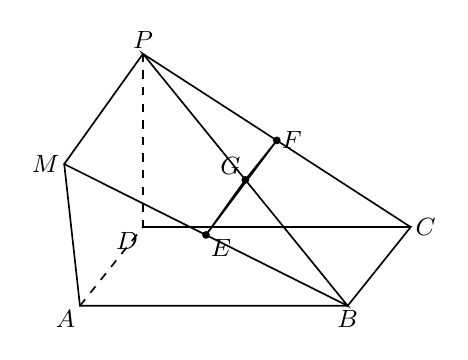
\begin{tikzpicture}[semithick, every node/.style={inner sep=1.5pt, font=\small}]
  \coordinate (A) at (0,0);
  \coordinate (B) at (3.4,0);
  \coordinate (C) at (4.2,1.0);
  \coordinate (D) at (0.8,1.0);
  \coordinate (M) at (-0.2,1.8);
  \coordinate (P) at (0.8,3.2);
  \coordinate (E) at (1.6,0.9);
  \coordinate (F) at (2.5,2.1);
  \coordinate (G) at (2.1,1.6);

  \draw (M) -- (A) -- (B) -- (C) -- (D);
  \draw (P) -- (M) -- (B) -- (P) -- (C);
  \draw[dashed] (P) -- (D);
  \draw[dashed] (A) -- (D);
  \draw (E) -- (F) -- (G) -- cycle;

  \fill (E) circle (1.4pt);
  \fill (F) circle (1.4pt);
  \fill (G) circle (1.4pt);
  \node[left] at (M) {$M$};
  \node[above] at (P) {$P$};
  \node[below left] at (A) {$A$};
  \node[below] at (B) {$B$};
  \node[right] at (C) {$C$};
  \node[below left] at (D) {$D$};
  \node[below right] at (E) {$E$};
  \node[right] at (F) {$F$};
  \node[above left] at (G) {$G$};
\end{tikzpicture}
\end{center}
\nopagebreak[4]
\end{question}
\endgroup
\begin{question}
\gkti{21}已知函数 $f(x)=\ln x-ax+\dfrac{1-a}{x}-1$（$a\in\mathbf R$）。

（1）当 $a=-1$ 时，求曲线 $y=f(x)$ 在点 $(2,f(2))$ 处的切线方程；

（2）当 $a\leqslant\dfrac12$ 时，讨论 $f(x)$ 的单调性。

\Needspace{0.4\textheight}
\end{question}
\begingroup
\renewenvironment{question}{\Needspace{0.5\textheight}}{}
\begin{question}
\gkti{22}如图，已知椭圆 $\dfrac{x^2}{a^2}+\dfrac{y^2}{b^2}=1$（$a>b>0$）过点 $\left(1,\dfrac{\sqrt2}2\right)$，离心率为 $\dfrac{\sqrt2}2$，左、右焦点分别为 $F_1$、$F_2$。点 $P$ 为直线 $l:x+y=2$ 上且不在 $x$ 轴上的任意一点，直线 $PF_1$ 和 $PF_2$ 与椭圆的交点分别为 $A$、$B$ 和 $C$、$D$，$O$ 为坐标原点。

（1）求椭圆的标准方程；

（2）设直线 $PF_1$、$PF_2$ 的斜率分别为 $k_1$、$k_2$。

① 证明：$\dfrac1{k_1}-\dfrac3{k_2}=2$；

② 问直线 $l$ 上是否存在点 $P$，使得直线 $OA$、$OB$、$OC$、$OD$ 的斜率 $k_{OA}$、$k_{OB}$、$k_{OC}$、$k_{OD}$ 满足 $k_{OA}+k_{OB}+k_{OC}+k_{OD}=0$？若存在，求出所有满足条件的点 $P$ 的坐标；若不存在，说明理由。
\nopagebreak[4]
\begin{center}% 2010 年山东卷文科第 22 题：椭圆、直线 l 与点 P。
% 来源 PDF：普通高考/2010/2010山东文.pdf，SHA-256 95a69b861a29ca594f9118c9643efcdfd04cae3c4f374ff9fa009f7ac99712f4。
% 原页：第 2 页（A3 三栏）第 3 栏上部，书页码 622。
% 重绘依据：椭圆 x^2/2+y^2=1，F1(-1,0)、F2(1,0)；l:x+y=2；
%   P(0.4,1.6) 在 l 上，PF1 交椭圆于 A、B，PF2 交椭圆于 C、D。
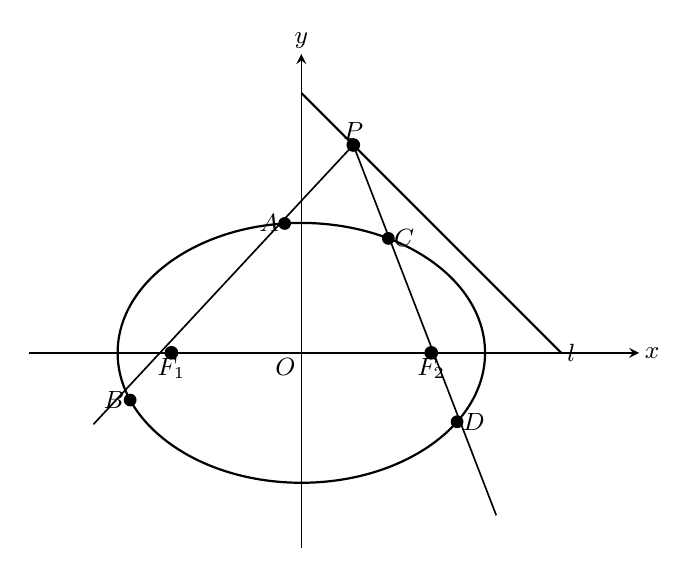
\begin{tikzpicture}[semithick, scale=1.65, every node/.style={inner sep=1.8pt, font=\small}]
  \draw[-stealth] (-2.1,0) -- (2.6,0) node[right] {$x$};
  \draw[-stealth] (0,-1.5) -- (0,2.3) node[above] {$y$};
  \draw[thick] (0,0) ellipse (1.414 and 1);
  \draw[thick] (0,2) -- (2,0) node[right] {$l$};
  \fill (-1,0) circle (1.5pt) node[below] {$F_1$};
  \fill (1,0) circle (1.5pt) node[below] {$F_2$};
  \fill (0.4,1.6) circle (1.5pt) node[above] {$P$};
  \draw (0.4,1.6) -- (-1.6,-0.55);
  \draw (0.4,1.6) -- (1.5,-1.25);
  \fill (-0.1286,0.9959) circle (1.4pt) node[left] {$A$};
  \fill (-1.3177,-0.3631) circle (1.4pt) node[left] {$B$};
  \fill (0.6697,0.8808) circle (1.4pt) node[right] {$C$};
  \fill (1.1989,-0.5304) circle (1.4pt) node[right] {$D$};
  \node[below left] at (0,0) {$O$};
\end{tikzpicture}
\end{center}
\nopagebreak[4]

\end{question}
\endgroup